\chapter{2020-05-26}

\section{Learn SWOW relation types as a mixture of ConceptNet's relation}
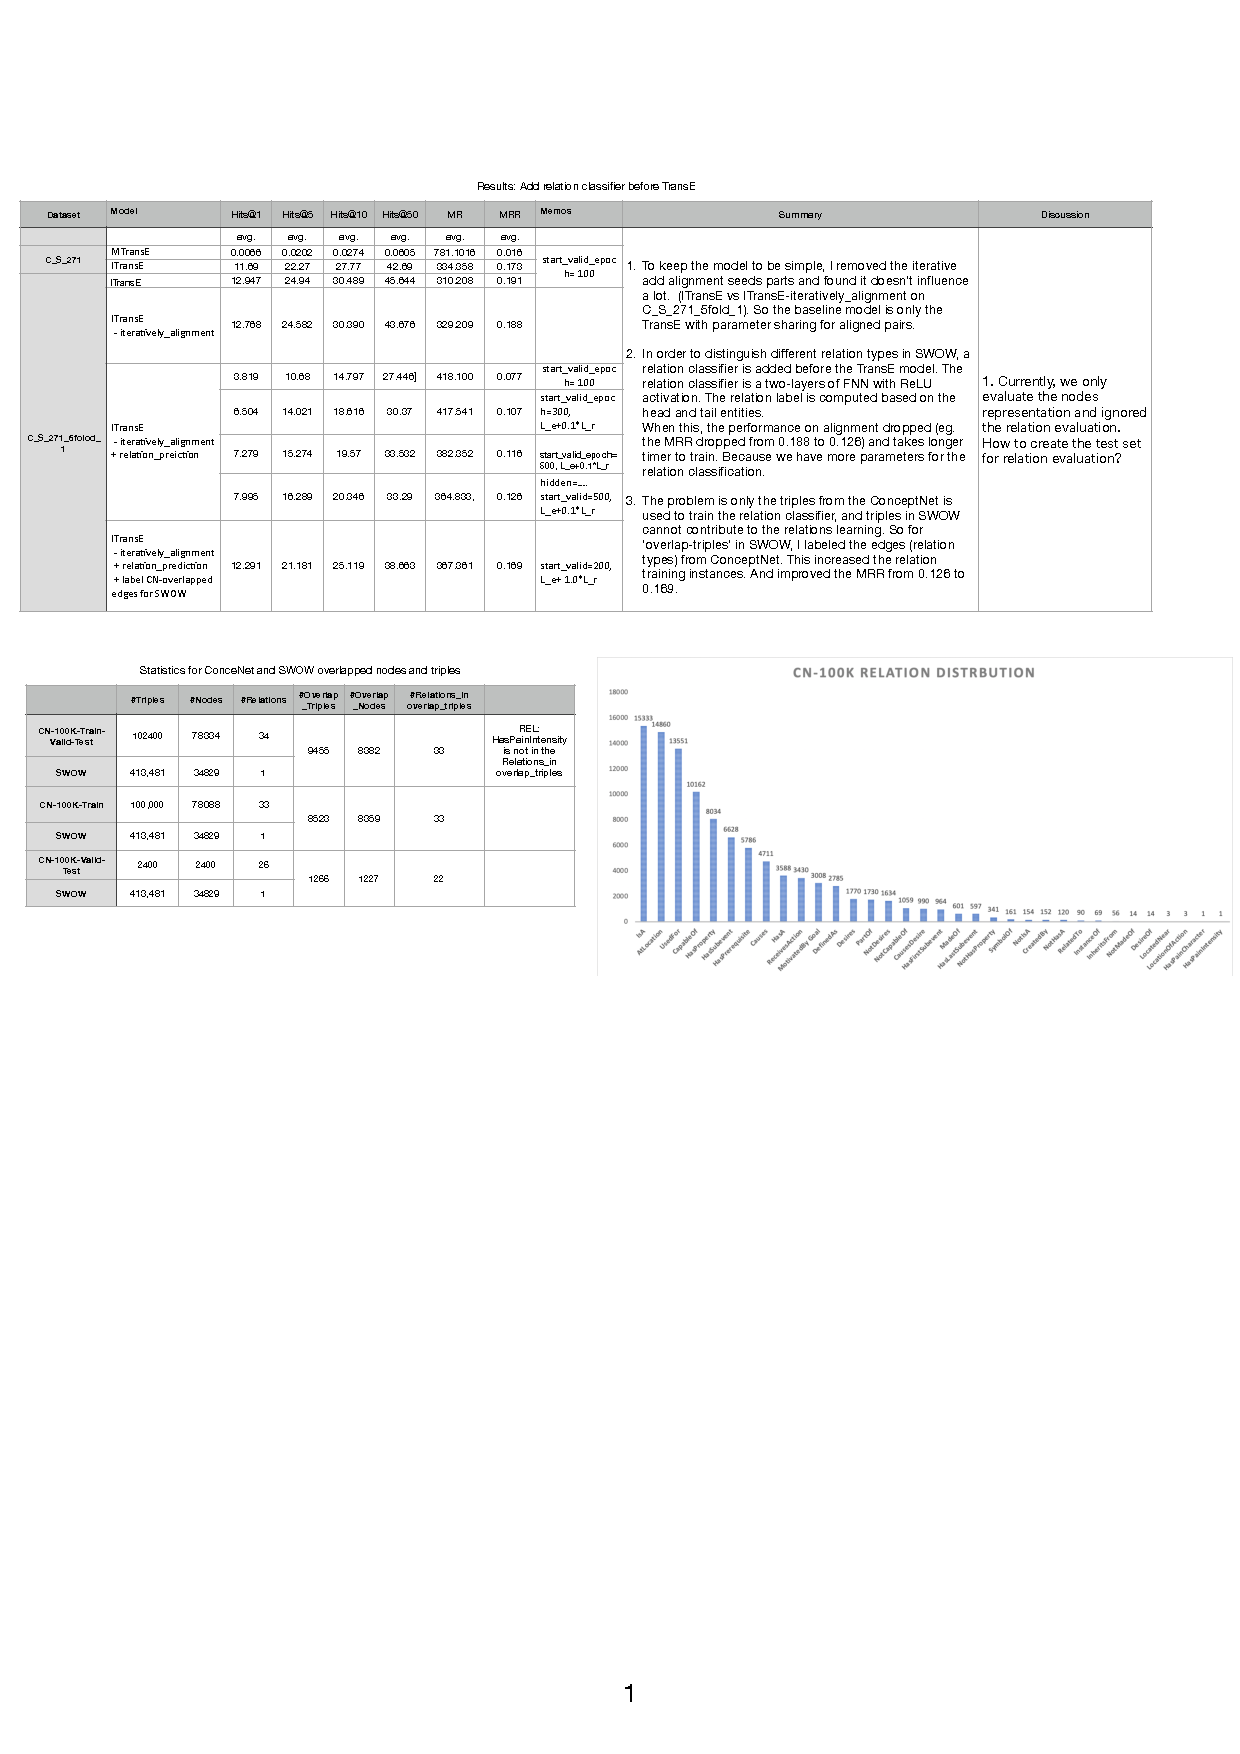
\includepdf[]{images/2020-05-26.pdf}

\section{Meeing Notes}
\textbf{To do list}
\begin{enumerate}
    \item Create test triples to evaluate learned relation embeddings (evaluate on relation type prediction).
    \item Loss modification: Add entropy constraint for relation distribution $\alpha$. We hope the $\alpha$ to be inclined to one label, so the entropy of $\alpha$ should be small. 
    \item Visualization: Use tensorboard to draw the training curves for loss $L_e$ and $L_r$, and use TSNE to visualize $\alpha$. (On both train and dev) 
    \item Maybe try different kinds of negative sampling strategy, eg., sample nodes with similar degeree or similar frequency. (But I am not really grasp why do we want this. How will this affect the model?)
   \item try learning a weight for the loss components
\end{enumerate}
Lea's comments: Regarding 4: we want this because by randomly sampling negative nodes we may make it too easy for the model to distinguish between true and fake triples. The fake ones will be completely implausible. We want to challenge the model by presenting it with plausible negative samples (somewhat like designing difficult multiple choice questions)

\begin{comment}
Relations id: {'LocationOfAction': 0, 'ReceivesAction': 1, 'HasPrerequisite': 2, 'MotivatedByGoal': 3, 'PartOf': 4, 'HasFirstSubevent': 5, 'HasProperty': 6, 'CreatedBy': 7, 'LocatedNear': 8, 'NotDesires': 9, 'HasSubevent': 10, 'DesireOf': 11, 'HasA': 12, 'InheritsFrom': 13, 'NotHasProperty': 14, 'HasPainIntensity': 15, 'CausesDesire': 16, 'RelatedTo': 17, 'NotMadeOf': 18, 'NotHasA': 19, 'InstanceOf': 20, 'Causes': 21, 'SymbolOf': 22, 'IsA': 23, 'HasPainCharacter': 24, 'UsedFor': 25, 'DefinedAs': 26, 'MadeOf': 27, 'AtLocation': 28, 'NotIsA': 29, 'NotCapableOf': 30, 'HasLastSubevent': 31, 'CapableOf': 32, 'Desires': 33} 

Relation counts from CN-100K (102400 triples total):

Relation count: [('HasPainCharacter', 1), ('HasPainIntensity', 1), ('LocatedNear', 3), ('LocationOfAction', 3), ('NotMadeOf', 14), ('DesireOf', 14), ('InheritsFrom', 56), ('
InstanceOf', 69), ('RelatedTo', 90), ('NotHasA', 120), ('CreatedBy', 152), ('NotIsA', 154), ('SymbolOf', 161), ('NotHasProperty', 341), ('HasLastSubevent', 597), ('MadeOf',
601), ('HasFirstSubevent', 964), ('CausesDesire', 990), ('NotCapableOf', 1059), ('NotDesires', 1634), ('PartOf', 1730), ('Desires', 1770), ('DefinedAs', 2785), ('MotivatedBy
Goal', 3008), ('ReceivesAction', 3430), ('HasA', 3588), ('Causes', 4711), ('HasPrerequisite', 5786), ('HasSubevent', 6628), ('HasProperty', 8034), ('CapableOf', 10162), ('Us
edFor', 13551), ('AtLocation', 14860), ('IsA', 15333)]



Loaded 377701 triples from ./data/alignment/C_S/rel_triples_1 with 30391 vocab
Total 37 relations.  Relation count: [('InstanceOf', 1), ('influencedBy', 1), ('SymbolOf', 3), ('EtymologicallyDerivedFrom', 6), ('NotCapableOf', 24), ('LocatedNear', 28), ('DefinedAs', 38), ('NotHasP
roperty', 112), ('CreatedBy', 135), ('HasFirstSubevent', 138), ('HasLastSubevent', 150), ('MadeOf', 281), ('CausesDesire', 311), ('Entails', 316), ('ReceivesAction', 418), ('Motiv
atedByGoal', 455), ('NotDesires', 512), ('Desires', 563), ('HasA', 822), ('HasPrerequisite', 886), ('DistinctFrom', 895), ('HasSubevent', 938), ('CapableOf', 971), ('Causes', 1078
), ('HasProperty', 1932), ('PartOf', 3146), ('UsedFor', 3998), ('Antonym', 4227), ('MannerOf', 8128), ('SimilarTo', 8225), ('AtLocation', 9659), ('FormOf', 11862), ('DerivedFrom',
 12778), ('IsA', 26499), ('HasContext', 30157), ('Synonym', 35660), ('RelatedTo', 212348)]


 Write 33 shared relations to ./data/alignment/C_S/rel_links                                                                                                               [51/1931]
Rel_links: {'Causes': 200, 'UsedFor': 1158, 'CausesDesire': 44, 'IsA': 2415, 'HasProperty': 1043, 'HasA': 326, 'MadeOf': 228, 'AtLocation': 2359, 'ReceivesAction': 147, 'PartOf': 
593, 'HasSubevent': 132, 'LocatedNear': 3, 'CapableOf': 280, 'NotCapableOf': 12, 'NotMadeOf': 4, 'HasLastSubevent': 12, 'InheritsFrom': 24, 'Desires': 65, 'HasPrerequisite': 136, 
'SymbolOf': 62, 'RelatedTo': 42, 'NotHasProperty': 32, 'MotivatedByGoal': 18, 'DefinedAs': 26, 'NotIsA': 19, 'CreatedBy': 35, 'NotDesires': 18, 'HasFirstSubevent': 3, 'LocationOfA
ction': 3, 'InstanceOf': 9, 'NotHasA': 4, 'DesireOf': 2, 'HasPainCharacter': 1}
\end{comment}
